\documentclass[11pt,a4paper]{article}

\usepackage[margin=2.3cm]{geometry}
\usepackage[T1]{fontenc}
\usepackage{mathpazo}
\linespread{1.05}
\usepackage{amsmath}
\usepackage{graphicx}
\usepackage{booktabs}
\usepackage{float}
\usepackage[font=small,labelfont=bf]{caption}
\usepackage{xcolor}
\usepackage[colorlinks=true,linkcolor=blue!50!black,urlcolor=blue!50!black]{hyperref}

\graphicspath{{figures/}}
\setlength{\parskip}{0.5em}
\setlength{\parindent}{0pt}

\title{\textbf{Signal Filtering: Results}}
\author{Aditya Sahai\\ \small M.Sc.\ Physics + B.E.\ Mechanical Engineering, BITS Pilani}
\date{October 2026}

\begin{document}
\maketitle

\section{Goal}
Compare four filters (moving average, low-pass, complementary and Kalman) on the same noisy sine wave.
Because the data is synthetic, the true signal is known, so each filter can be scored exactly.
The filters will later be used on real MPU-6050 data in a separate project.

\section{Setup}

\textbf{Data.}
\begin{itemize}
  \item True signal: $2\sin x$, with 101 points from $0$ to $2\pi$ (step $\Delta x = 0.0628$\,rad).
  \item Noisy position (like an accelerometer): true signal $+$ uniform noise of width 1.0.
  \item Rate (like a gyroscope): $2\cos x$ $+$ a constant bias $+$ a little noise.
  \item Calibration: 200 readings taken while ``still'', used to find the bias, $R$ and $Q$.
\end{itemize}

\textbf{Filter settings.}
\begin{itemize}
  \item Moving average with $N = 10$ and low-pass with $\alpha = 0.82$. These two were chosen to have the
        same lag in theory, so they can be compared fairly.
  \item Complementary with $\beta = 0.975$.
  \item Kalman, with the bias, $R$ and $Q$ found from calibration.
\end{itemize}

\textbf{Metrics.}
\begin{itemize}
  \item \textbf{RMSE:} the average size of the error between the filtered and true signal. Lower is better.
  \item \textbf{Lag:} how far the filtered signal trails behind the true signal.
  \item \textbf{Residual noise:} how much noise is left once the lag is removed.
  \item \textbf{Attenuation:} how tall the filtered wave is compared with the true one (1 = full height).
\end{itemize}

\section{Results}
All filters were run on the same data (random seed 42).

\begin{table}[H]
\centering
\caption{Results for seed 42.}
\begin{tabular}{lcccc}
\toprule
Signal & RMSE & Lag (rad) & Residual noise & Attenuation \\
\midrule
Raw (no filter)            & 0.297 & 0.000 & 0.297 & 1.168 \\
Moving average ($N=10$)    & 0.402 & 0.314 & 0.105 & 0.999 \\
Low-pass ($\alpha=0.82$)   & 0.378 & 0.251 & 0.121 & 0.988 \\
Complementary ($\beta=0.975$) & \textbf{0.059} & 0.000 & \textbf{0.059} & 0.983 \\
Kalman                     & 0.095 & 0.000 & 0.082 & 0.965 \\
\bottomrule
\end{tabular}
\end{table}

\begin{figure}[H]
\centering
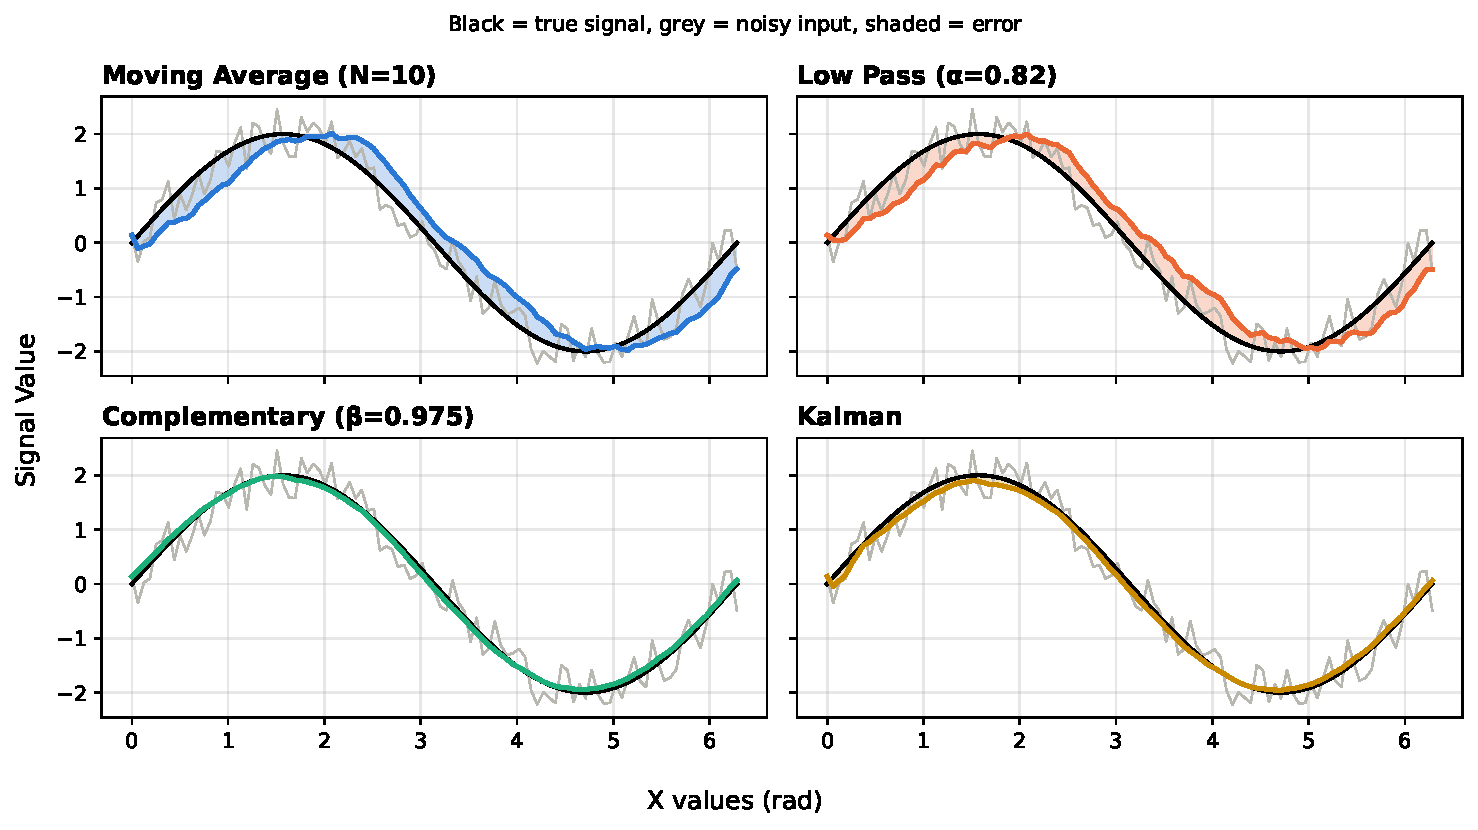
\includegraphics[width=\linewidth]{small_multiples.pdf}
\caption{Each filter in its own panel. Black is the true signal, grey is the noisy input and the coloured line is
the filter's output. The shaded area between the coloured line and the black line is the filter's error.}
\label{fig:panels}
\end{figure}

\textbf{What Figure~\ref{fig:panels} shows.} All four panels use the same axes, so they can be compared directly.
\begin{itemize}
  \item \textbf{Moving average and low-pass (top row):} the coloured curve is smooth but sits to the \emph{right}
        of the black line, so it is \emph{late}. When the signal is rising the filter reads too low, and when it
        is falling it reads too high. That gap is the large shaded area, up to about 0.6 at its widest.
  \item \textbf{Complementary and Kalman (bottom row):} the coloured curve sits almost on top of the black line,
        so there is very little shading. These filters are smooth \emph{and} on time.
\end{itemize}

\textbf{Main finding.} The moving average and low-pass filters remove most of the noise (residual noise drops from
0.30 to about 0.11), but they are so late that their RMSE is \emph{worse} than doing nothing (0.38--0.40 vs 0.30).
The complementary and Kalman filters use the rate to predict where the signal is going, so they remove the noise
\emph{without} being late.

\section{Theory vs.\ Measured}
The formulas below are the ones from my notes. $\sigma$ is the noise level of the raw signal; for uniform noise
of width $w$, $\sigma = w/\sqrt{12} = 0.289$.

\begin{table}[H]
\centering
\caption{Theoretical values against measured values.}
\begin{tabular}{llcc}
\toprule
What & Formula & Theory & Measured (seed 42) \\
\midrule
Raw noise                     & $w/\sqrt{12}$                      & 0.289        & 0.297 \\
Moving average lag            & $(N-1)/2$ samples                  & 4.5 samples  & 5 samples \\
Low-pass lag                  & $\alpha/(1-\alpha)$ samples        & 4.6 samples  & 4 samples \\
Moving average noise          & $\sigma/\sqrt{N}$                  & 0.091        & 0.105 \\
Low-pass noise                & $\sigma\sqrt{(1-\alpha)/(1+\alpha)}$ & 0.091      & 0.121 \\
Calibrated $R$                & $w^2/12$                           & 0.0833       & 0.0802 \\
Calibrated bias               & true bias                          & 0.1802       & 0.1816 \\
Final Kalman gain $K$ vs.\ $1-\beta$ & ---                         & 0.025        & 0.026 \\
\bottomrule
\end{tabular}
\end{table}

\textbf{Why the small differences?}
\begin{itemize}
  \item \textbf{Lag} is measured in whole samples, so a theoretical 4.5 or 4.6 can only show up as 4 or 5.
        Both are within one sample of theory.
  \item \textbf{Low-pass noise} comes out a little high for the same reason: its lag of 4.6 samples can only be
        removed as 4 whole samples, so the leftover shift is counted as noise.
  \item \textbf{Raw noise, $R$ and the bias} differ slightly because they are estimated from a limited number of
        random samples.
  \item \textbf{Kalman gain:} the Kalman filter worked out its own gain from $R$ and $Q$ and ended up at 0.026,
        almost exactly the $1-\beta = 0.025$ I chose by hand for the complementary filter.
\end{itemize}

\section{How the Kalman Gain Changes}

\begin{figure}[H]
\centering
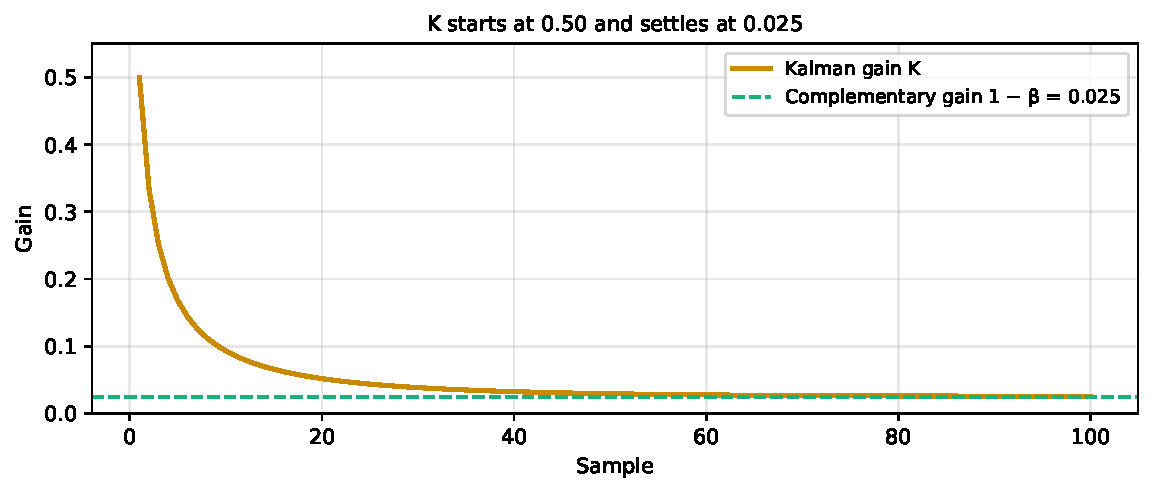
\includegraphics[width=0.95\linewidth]{kalman_gain.pdf}
\caption{Kalman gain $K$ at each step (yellow) and the complementary filter's fixed gain $1-\beta$ (green dashed).}
\label{fig:gain}
\end{figure}

\textbf{What Figure~\ref{fig:gain} shows.} The gain is the weight given to each new measurement. The Kalman filter
starts with $K = 0.5$: at the beginning it is unsure of its estimate, so it trusts the measurements a lot. As it
gains confidence, $K$ drops and settles at about 0.026. The complementary filter uses the same small gain (0.025)
from the very first sample.

\section{Repeating the Test with 50 Different Noise Patterns}
One run uses one random noise pattern, which could be lucky or unlucky. So the whole test was repeated with
50 different random seeds (0 to 49) and the results were averaged.

\begin{figure}[H]
\centering
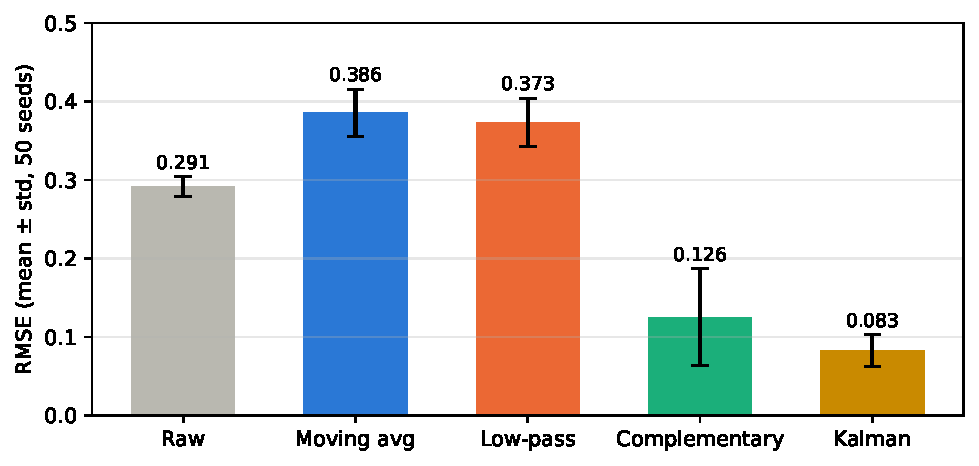
\includegraphics[width=0.8\linewidth]{rmse_seeds.pdf}
\caption{Average RMSE over 50 runs. The bar is the average; the thin line shows how much it varies between runs.}
\label{fig:seeds}
\end{figure}

\textbf{What Figure~\ref{fig:seeds} shows.} On average, the Kalman filter has the lowest error (0.083) and varies
the least between runs. The complementary filter is second (0.126) but varies a lot. The moving average and
low-pass filters are worse than the raw signal in all 50 runs.

\textbf{Why this differs from seed 42.} With seed 42 the complementary filter came first, but over 50 runs the
Kalman filter wins 36 times. The reason is how they start. Both filters begin from the first noisy reading. If
that reading is badly off:
\begin{itemize}
  \item the complementary filter fixes it slowly, because its gain is always small (0.025);
  \item the Kalman filter fixes it within a few samples, because its gain starts large (0.5), as Figure~\ref{fig:gain} shows.
\end{itemize}
In seed 42 the first reading happened to be quite accurate, so the complementary filter's slow start did not hurt it.

\section{Conclusions}
\begin{enumerate}
  \item \textbf{Moving average and low-pass filters remove noise but add lag.} On a changing signal, the lag
        costs more than the noise they remove, so their total error is worse than no filter.
  \item \textbf{Using the rate removes the lag.} The complementary and Kalman filters predict where the signal is
        going, so they smooth the signal without falling behind. They cut the error by about 55--70\%.
  \item \textbf{The Kalman filter is the most reliable.} It found almost the same gain I picked by hand, and its
        large starting gain lets it recover quickly from a bad first reading.
  \item \textbf{The results agree with theory}, within one sample for lag and within a few percent for noise.
\end{enumerate}

\textbf{Future work:} test other signal speeds and filter settings, test a sudden step, and apply the filters to
real MPU-6050 data.

\end{document}